\section{Controladores \glsentryshort{sdn}}
\label{sec:sdnControllers}

Los controladores \gls{sdn}, también conocidos como sistemas operativos de red, son una pieza cable en los entornos  \gls{sdn} dado que tienen una vista global de toda la red que gestionan, que flujos atraviesan la red, estadísticas, usuarios finales, modelos y características de dichos equipos. Este controlador tiene la funcionalidad de interconectar los recursos disponibles en la red que gestiona, a aplicaciones o servicios que corran encima de él \cite{nadeau2013sdn}. De esta forma, cada vez que se quiera añadir una nueva funcionalidad, solo se tendrá que programar un nuevo servicio que corra encima del controlador que gestiona la red, y este a su vez se encargará de traducir las demandas del servicio a políticas de red a cada dispositivo impactado. En este matiz se puede llegar apreciar el sentido de nombre del paradigma \gls{sdn}, ya que estamos definiendo por software el comportamiento intrínseco de la red.\\
\\
% fig
\begin{figure}[ht]
    \centering
    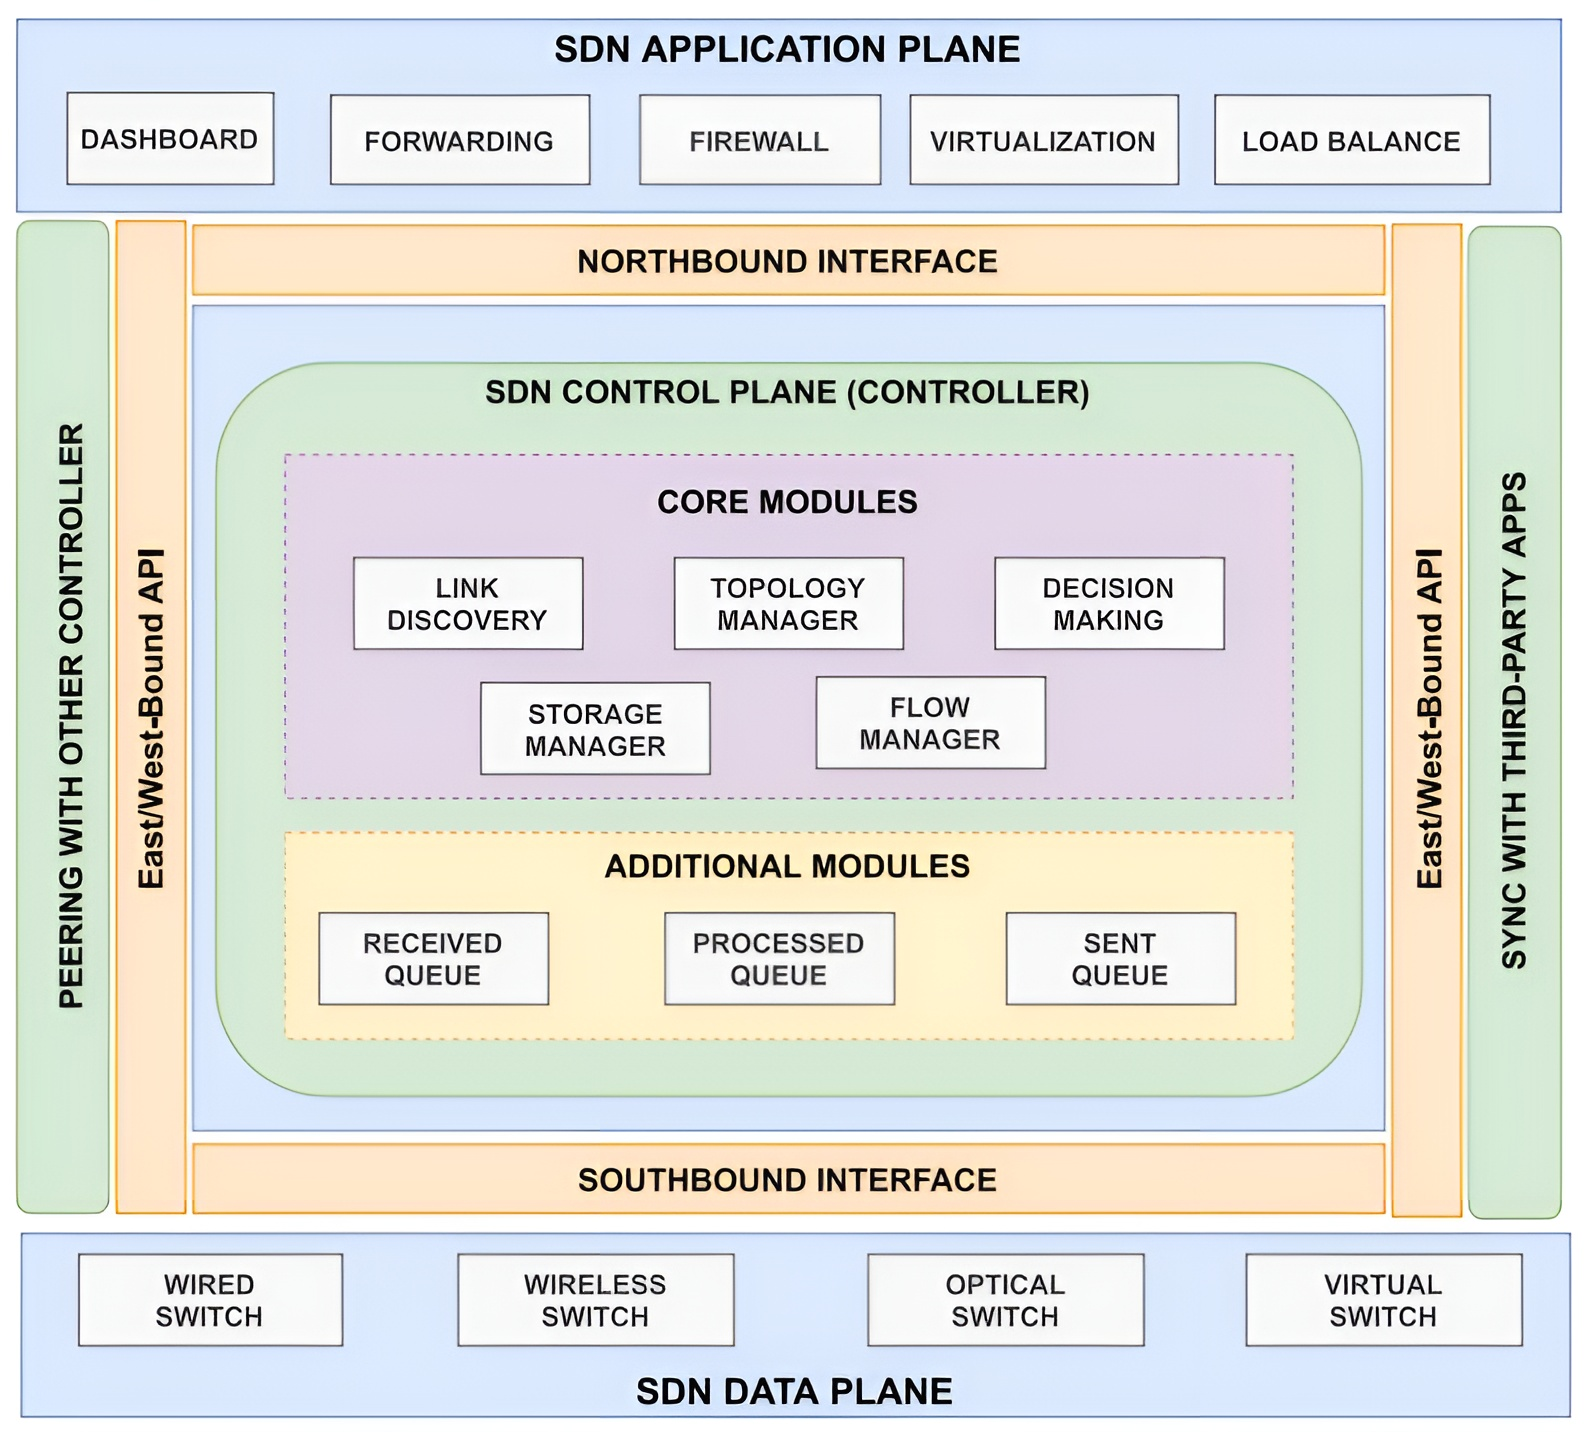
\includegraphics[width=\textwidth]{archivos/img/teoria/sdn_controllers.jpg}
    \caption{Arquitectura generica de controlador \gls{sdn} \cite{zhu2020sdn}}
    \label{fig:sdn_controllers}
\end{figure}

En la literatura hay muchas propuestas de arquitecturas para los controladores, pero en vez de ir una por una viendo las diferencias vamos a presentar la arquitectura genérica que se puede encontrar en la gran mayoría de controladores \gls{sdn}. Si nos fijamos en la figura \ref{fig:sdn_controllers}, podemos ver dos partes claramente diferenciadas, el núcleo del controlador y las interfaces del mismo \cite{zhu2020sdn}. Empezando por el \textit{core}, se puede resumir que las funciones básicas del controlador están relacionadas principalmente con el descubrimiento de la topología y la gestión de los flujos de tráfico. El módulo de descubrimiento de la topología suele trabajar con el protocolo \gls{lldp}. La implementación puede variar entre controladores y aplicaciones de descubrimiento topológico, pero en términos generales, se transmite regularmente consultas utilizando mensajes \texttt{packet\_out}, los cuales viajaran por la topología física y volverán al controlador en forma de mensajes \texttt{packet\_in}, que permiten al controlador construir la topología de la red.\\
\\
Una vez que se conoce la topología de red, el controlador puede empezar a poner en marcha distintos módulos de toma de decisiones para encontrar los caminos óptimos entre los nodos de la red. Con todos los caminos ya construidos, entran en juego otros módulos del controlador como son \gls{qos} y de seguridad, los cuales pueden optar por instalar una ruta sub-óptima para satisfacer los criterios de \gls{qos} o de seguridad. De forma adicional, el controlador puede tener un recopilador de estadísticas y un gestor de colas para recopilar información sobre el rendimiento de las diferentes colas de paquetes entrantes y salientes de los dispositivos de red que gestiona, y con ellos realimentar a los módulos de \gls{qos}. Por último, tenemos uno de los módulos más importantes del controlador, el gestor de flujos. El gestor de flujos, puede variar su implementación en función de los protocolos que se utilicen en la \gls{sbi}, pero su misión es la misma, instalar reglas en los dispositivos de red que gestiona las directrices necesarias para gestionar los paquetes de un determinado flujo de una determinada manera. \\
\\
Siguiendo con otra parte fundamental del controlador \gls{sdn} genérico, son las interfaces. El controlador está rodeado de interfaces para interactuar con otras capas, superior e inferior, y otros controladores, este y oeste (E-WBIs). Empezando por la interfaz \gls{sbi}, la cual es la encargada de interconectar dispositivos \gls{sdn} con el controlador, define un conjunto de reglas, que variarán en función del protocolo que se utilice, las cuales permiten definir el procesamiento y las políticas de reenvío de los dispositivos \gls{sdn}. El protocolo OpenFlow es unas de las \gls{sbi} más utilizadas, y es un estándar de facto para la industria, con el cual podemos es definir flujos y clasificar el tráfico de red basándose en un conjunto de reglas predefinidas. Pero también se pueden encontrar otras \gls{sbi}, como por ejemplo, P4Runtime de facto el futuro para las \gls{sbi}s, o podemos encontrar algunas más \textit{legacy}, como por ejemplo, Netconf o incluso \gls{snmp}.\\
\\
Si nos vamos de la API sur, al norte, encontraremos la conocida como \gls{nbi}, la cual interconecta el controlador \gls{sdn} con las aplicaciones de los desarrolladores o los servicios que definan el comportamiento intrínseco de la red. Los controladores admiten varias interfaces de programación de aplicaciones (API) northbound, pero la mayoría de ellas se basan en la API REST. Generalmente se quiere que la interfaz \gls{nbi} sea una interfaz genérica para que limite a los desarrolladores. Para la comunicación entre controladores, se utilizan las interfaces conocidas como de este y oeste (E/WBI), las cuales no tienen una interfaz de comunicación estándar, por lo que, en función del controlador se tendrá una implementación u otra.\\
\\
A continuación, se van a ir presentando algunos de los controladores \gls{sdn} más conocidos, indicando algunas de sus virtudes y funcionamiento en particular.

\subsection{Ryu}
\label{subsec:ryu}

Ryu\footnote{Del Japonés, significa "flujo" y también "dragón", ambos símbolos Kanji se leen igual como RYU, de ahí que el logo sea un dragón.} es un controlador de red de código abierto diseñado específicamente para redes \gls{sdn}. Se desarrolló en Python por el equipo de NTT (\textit{Nippon Telegraph and Telephone}) y proporciona una plataforma flexible, sencilla y extensible para desarrollar aplicaciones de red basadas en SDN. Como se comentó anteriormente, la funcionalidad primordial que lleva a cabo es la de ser un intermediario entre los elementos de red, como por ejemplo switches SDN o nodos virtuales, y las aplicaciones o servicios que controlan la red a través de la \gls{nbi} \cite{tomonori2013introduction}. De esta forma, a través de la \gls{nbi}, permite a los desarrolladores programar el comportamiento de la red de manera dinámica y centralizada, facilitando la implementación de políticas de red, la configuración de routing y la gestión de tráfico.\\
\\
Ryu es altamente modular y proporciona una API bien definida que permite a los desarrolladores construir aplicaciones de red personalizadas hasta el más mínimo nivel. También es compatible con varios protocolos de comunicación utilizados en SDN, como OpenFlow (versiones \texttt{1.0, 1.2, 1.3, 1.4, 1.5}), NETCONF y OF-config \cite{tomonori2013introduction}.  Las aplicaciones Ryu son entidades que implementan varias funcionalidades dentro de Ryu y se comunican entre sí a través de eventos. Los eventos sirven como mensajes intercambiados entre las aplicaciones Ryu. Estas aplicaciones se envían eventos asíncronos entre sí, creando un flujo de comunicación. Además de las aplicaciones Ryu, existen ciertas fuentes de eventos internas al propio Ryu. Un ejemplo de estas fuentes de eventos es el controlador OpenFlow. Cada aplicación Ryu posee una cola de recepción específicamente diseñada para eventos. La cola funciona según el principio \gls{fifo}, lo que garantiza que se mantenga el orden de los eventos. Para procesar estos eventos, cada aplicación Ryu tiene un único hilo dedicado responsable de la gestión de eventos. Este subproceso vacía continuamente la cola de recepción retirando los eventos de la cola e invocando al manejador de eventos apropiado en función del tipo de evento \cite{ryu1}.

\newpage

% fig
\begin{figure}[ht]
    \centering
    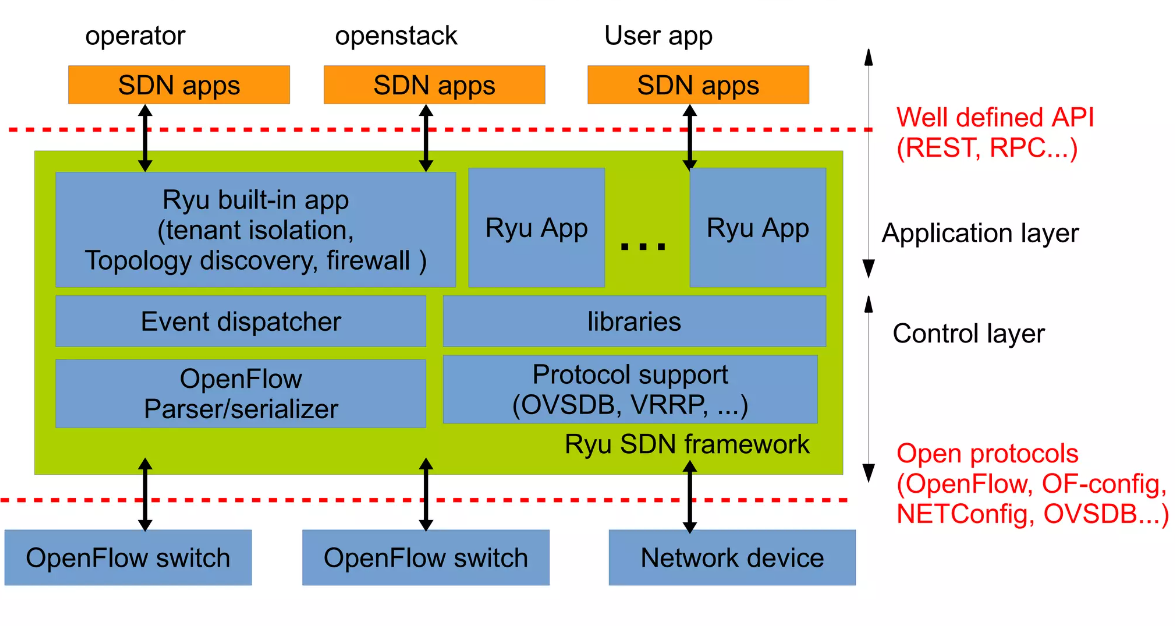
\includegraphics[width=0.85\textwidth]{archivos/img/teoria/ryu.png}
    \caption{Arquitectura del controlador \gls{sdn} RYU \cite{ryu2}}
    \label{fig:ryu}
\end{figure}

En la figura \ref*{fig:ryu}, se puede apreciar como la arquitectura del controlador está divida en dos grandes bloques de acuerdo se han estudiado los controladores \gls{sdn}, la parte de \textit{core} y la parte de interfaces. En la parte del núcleo se puede apreciar como se a programado todas las librerías y el manejador de eventos que se mencionaba anteriormente. Por otro lado también se puede apreciar las capas de adaptación a la \gls{sbi} y a la \gls{nbi}, la primera de ellas se adapta a través de una API REST a servicios de aplicaciones externas, mientas que la interfaz \gls{sbi} implementa todos los protocolos de control \gls{sdn}. Algunas de las características y funcionalidades de Ryu incluyen:

\begin{itemize}
    \item Compatibilidad con múltiples protocolos SDN de la interfaz \gls{sbi}.
    \item Capacidad para implementar políticas de red y reglas de enrutamiento de forma sencilla.
    \item Soporte para la recopilación y el análisis de datos de red en tiempo real.
    \item Funcionalidad de control de \gls{qos}.
    \item La más importante de todas, fácil desarrollo y portabilidad sencilla al estar escrita en Python. Esta última se puede ver también como una desventaja, dado el pobre rendimiento de un lenguaje interpretado.
\end{itemize}

Ryu es utilizado en una amplia gama de entornos, desde laboratorios de investigación hasta en las clases de forma educativa. Esta herramienta suele ser el punto de estrada para muchas personas que se inician en el \gls{sdn}, sin embargo, al tener un pobre rendimiento, en entornos comerciales no se suele ver con tanta frecuencia \cite{tomonori2013introduction}.

\subsection{ONOS}
\label{subsec:ONOS}

\gls{onos} es un controlador de red de código abierto diseñado específicamente para redes \gls{sdn}. Como su nombre indica, \gls{onos} es un sistema operativo para redes que proporciona funcionalidades avanzadas de control y gestión de redes. \gls{onos} está diseñado para ser escalable, confiable y de alto rendimiento, lo que lo hace adecuado para despliegues de red a gran escala. Es compatible con una amplia variedad de protocolos y tecnologías de red, como OpenFlow, NETCONF, BGP y \gls{p4}. El controlador está respaldado por la \gls{onf}, la cual es una una organización sin ánimo de lucro fundada en 2011 con el objetivo de promover y acelerar la adopción de la tecnología \gls{sdn} y el enfoque de redes abiertas. Además de la \gls{onf}, numerosos provedores de internet están impulsando el proyecto, así como, grandes empresas del sector TIC. Se pueden resumir las principales características y funcionalidades de \gls{onos} en los siguientes puntos.

\begin{itemize}
    \item  Control centralizado de la red: \gls{onos} proporciona un punto central de control para la gestión de toda la red. Permite la configuración dinámica de la red, el enrutamiento y la asignación de recursos.
    \item Escalabilidad: \gls{onos} está diseñado para manejar redes de gran escala, distribuyendo la carga de trabajo entre múltiples nodos para lograr un rendimiento óptimo y una alta disponibilidad.
    \item Programabilidad: \gls{onos} permite a los desarrolladores crear aplicaciones personalizadas utilizando una amplia gama de APIs y marcos de desarrollo. Esto facilita la implementación de políticas de red, la orquestación de servicios y la integración con otras aplicaciones y sistemas.
    \item Gestión de topología: \gls{onos} proporciona una visión global de la topología de la red, permitiendo el descubrimiento de dispositivos, enlaces y rutas. Esto facilita la toma de decisiones basadas en el estado actual de la red.
    \item Gestión de flujos: \gls{onos} admite la programación y gestión de flujos de red, lo que permite la implementación de políticas de enrutamiento y \gls{qos} de manera dinámica y centralizada.
    \item Segmentación de red: \gls{onos} es compatible con la segmentación de red, lo que permite crear \textit{network slices} para proporcionar aislamiento y asignación de recursos personalizada en una infraestructura compartida.
\end{itemize}

\gls{onos} se concibe como un sistema operativo de red completo que va más allá de ser solo un controlador \gls{sdn}. Ofrece una amplia gama de funcionalidades que incluyen herramientas como APIs que proporcionan abstracción para el desarrollo de aplicaciones \gls{sdn}, así como APIs para la administración, supervisión y programación de dispositivos de red. Además, \gls{onos} ofrece capacidades de virtualización, aislamiento, acceso seguro y abstracción de los recursos de red administrados por el sistema operativo. \gls{onos} tiene la capacidad de multiplexar recursos tanto hardware como software entre las aplicaciones \gls{sdn}, permitiendo una utilización eficiente de los recursos disponibles. Además, facilita la configuración de políticas de red basadas en las intenciones de las aplicaciones, lo que implica la aplicación de políticas de red diseñadas para satisfacer los requisitos específicos de las aplicaciones, así como el procesamiento de eventos de red. \\
\\
Si nos fijamos en la figura \ref*{fig:onos}, podemos ver que este sistema operativo está diseñado para operar con dispositivos de red \textit{whitebox}, con el objetivo de reducir los costes asociados con las soluciones propietarias. \gls{onos} posee una arquitectura flexible que facilita la integración sencilla de nuevos dispositivos de hardware en el framework \gls{sdn}. Solo se requiere que se añada un driver del equipo o target propietario.  Además, puede funcionar como un sistema distribuido a través de múltiples servidores en modo cluster, lo que permite aprovechar los recursos de CPU y memoria de varios equipos simultáneamente. Esta capacidad también proporciona resilencia ante posibles fallos de los servidores y permite realizar cambios en hardware y software sin interrumpir el tráfico de red.

% fig
\begin{figure}[ht]
    \centering
    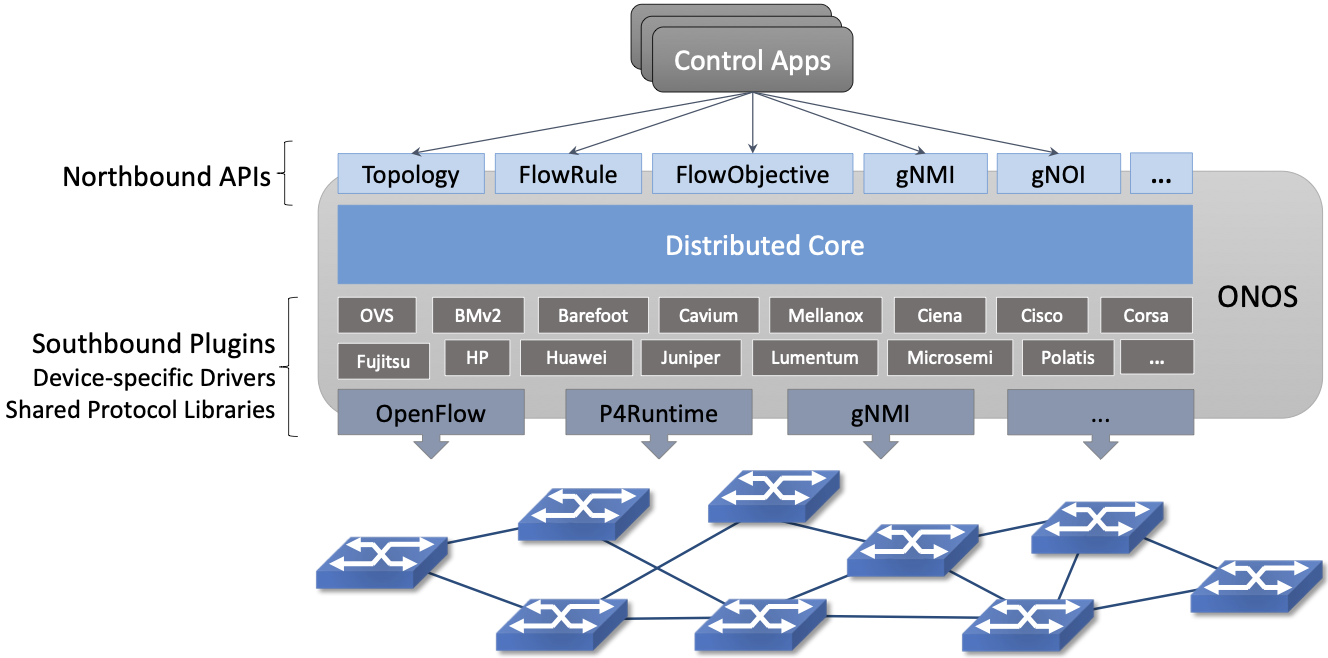
\includegraphics[width=\textwidth]{archivos/img/teoria/onos.png}
    \caption{Arquitectura del controlador \gls{sdn} onos \cite{ryu2}}
    \label{fig:onos}
\end{figure}

\gls{onos} cuenta con una comunidad activa de desarrolladores y usuarios que contribuyen al desarrollo y mejora del sistema. Además, \gls{onos} es utilizado en diversos casos de uso, como redes de transporte, redes de centros de datos y redes de telecomunicaciones, entre otros muchos casos de uso. Si bien es cierto que tiene un muy buen rendimiento, no es controlador sencillo de manejar, y la curva de aprendizaje puede ser bastante pronunciada.